\chapter{Lecture 20 - Gauss Quadrature}
\label{ch:lec20n}
\section{Objectives}
The objectives of this lecture are to:
\begin{itemize}
\item Define Gauss-Legendre quadrature and illustrate its convergence properties
\item Provide a derivation to explain how and why Gauss quadrature works
\end{itemize}
\setcounter{lstannotation}{0}

\section{Gauss-Legendre Quadrature}
Gauss-Legendre quadrature, from here-on-out referred to simply as Gauss quadrature, is similar to Newton-Cotes integration formulas in its overall algorithmic strategy:
\begin{itemize}
\item Approximate $f(x)$ by some other function, $g(x)$, that is in some way ``close'' to $f(x)$; and
\item Integrate that function exactly.
\end{itemize}
The main differences are:
\begin{enumerate}
\item Gauss quadrature schemes use a different measure to determine if $g(x)$ is ``close'' to $f(x)$.  In Newton-Cotes formulas, $g(x)$ was forced to be equal to $f(x)$ at pre-selected locations.  Gauss quadrature measures closeness in an integral sense as shown in Equation \ref{eq:lec20n-gq-close}.
\begin{equation}
\int_{a}^{b}\left[f(x) - g(x)\right]g(x) \ dx = 0
\label{eq:lec20n-gq-close}
\end{equation}
\marginnote[-1.0cm]{If $g(x)$ is close to $f(x)$, then the integral in Equation \ref{eq:lec20n-gq-close}, which we can think of as an inner product between $g(x)$ and the ``error'' $f(x) - g(x)$, will be small.}
\item Gauss quadrature does not require $g(x)$ to match $f(x)$ at any pre-determined number of locations in the interval, but it does call for sampling $f(x)$ at a number of discrete points throughout the interval much like trapezoidal and Simpson's rule does.  The location of these sample points (often called \emph{integration points} or \emph{Gauss points}) is a key factor to the accuracy that Gauss quadrature can achieve.
\end{enumerate}

In this lecture we will discuss two versions of the Gauss quadrature algorithm.  First, we will describe the algorithm in a recipe-like way without any discussion regarding the theory as to why it all works.  After that is out of the way, a full derivation will be presented so that readers will know exactly how and why the method works.

\section{The Short Version}
In Gauss quadrature, the definite integral of a function $f(x)$ over an interval $[-1,1]$ is approximated by Equation \ref{eq:lec20n-gq-short}.
\begin{equation}
\int_{-1}^{1} f(x) \ dx \approx \sum\limits_{i=1}^{N}w_i f(x_i)
\label{eq:lec20n-gq-short}
\end{equation}
Since we generally do not want to integrate functions only from $x\in[-1,1]$, we will linearly map the desired domain, $[a,b]$ onto the reference domain, $t \in [-1,1]$ as follows:\marginnote{Notice that at $x(t=-1) = a$, and $x(t=1) = b$.}
\begin{align*}
x(t) &= \frac{1}{2}\left[(b-a)t + a + b \right] \\
dx &= \frac{1}{2}(b-a) \ dt
\end{align*}
Substituting this into the equation above gives us:
\begin{equation}
\int_{a}^{b}f(x) \ dx = \int_{-1}^{1}f(x(t))\frac{b-1}{2} \ dt \approx \sum\limits_{i=1}^{n}w_i f(x(t_i))\frac{b-a}{2}
\label{eq:lec20n-gp-formula}
\end{equation}

\begin{marginfigure}
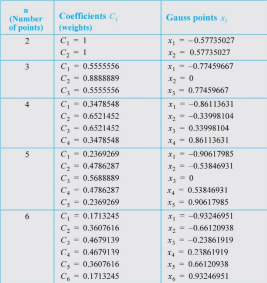
\includegraphics{lec20n-gp-and-weights.png}
\caption{Published Gauss points and weights up to $n=6$.}
\label{fig:lec20n-gp-and-weights}
\end{marginfigure}
Values for Gauss points and weights are commonly tabulated, as shown in Figure \ref{fig:lec20n-gp-and-weights}. Engineers wanting to use Gauss quadrature incorporate those values into their code in some appropriate way and carry out the numeric integration.

The convergence of Gauss quadrature depends on the number of Gauss points used: order $2n-1$ for $n$ points.  If you want faster convergence, simply add more points.\sidenote{This is referred to as \emph{exponential convergence.}}  Figure \ref{fig:lec20n-gq-convergence} shows the convergence behavior of Gauss quadrature for calculating the integral:
\begin{equation*}
\int_{-3}^3 e^{-x^2} \ dx
\end{equation*}
\begin{marginfigure}
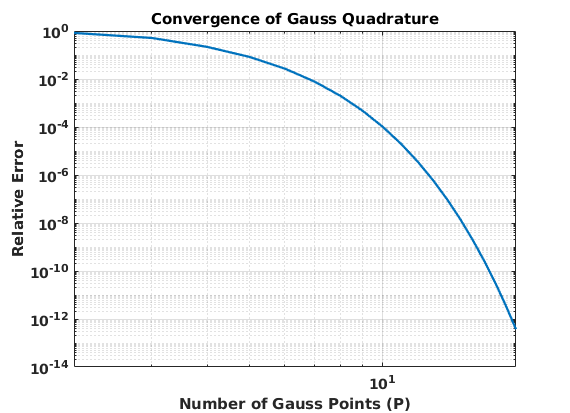
\includegraphics{lec20n-gq-convergence.png}
\caption{Convergence behavior of Gauss quadrature.}
\label{fig:lec20n-gq-convergence}
\end{marginfigure}
This convergence result was obtained using a single interval for the integral.  It is, of course, possible to break the domain into multiple sub-domains and carry out the integral using Gauss quadrature for each sub-domain and then sum the result.  In that case, convergence depends on the number of Gauss points used on each sub-domain.  The error will be $\mathcal{O}(h^{2n-1})$ where $h$ is the size of each sub-domain and $n$ is the number of Gauss points used on each sub-domain.


\section{The Long Version}

For Gauss quadrature, we approximate the integral of $f(x)$ as follows:
\begin{equation*}
\int_{a}^{b} f(x) \ dx \approx \sum\limits_{i=1}^{n}w_i g(x_i)
\end{equation*}
where, as before, $w_i$ are the weights and $x_i$ are the sample points.  We are free to choose these weights and sample points in any way we wish, giving us a total of $2n$ degrees of freedom.

With these $2n$ degrees of freedom, we might hope to \emph{exactly} integrate any polynomial up to degree $2n-1$ much like in the trapezoidal and Simpson's rule.  The key is to choose the sample points and weights carefully so that we can achieve this goal.

For Gauss-Legendre quadrature, we will choose the functions $g(x)$ to be Legendre polynomials.\sidenote{This is why our method is called \emph{Gauss-Legendre} quadrature. There are several other variations of Gauss quadrature that use other sets of orthogonal polynomials but the theory presented in this lecture is typical.}  Legendre polynomials were first introduced in Lecture 9 of the analytical methods portion of this text.  As a review, Legendre polynomials, $P_n(x)$, are solutions to Legendre's differential equation:
\begin{equation}
\frac{d}{dx}\left[\left(1-x^2\right)\frac{d}{dx}P_n(x)\right] + n(n+1)P_n(x) = 0, \ \ n=0,1,2,\dots
\end{equation}
The first two Legendre polynomials are:
\begin{equation*}
P_0(x) = 1 \ \ \ P_1(x) = 1
\end{equation*}
and subsequent polynomials can be found using a 3-term recurrence relation:
\begin{equation}
(n+1)P_{n+1}(x) = (2n+1)xP_n(x)-nP_{n-1}(x)
\end{equation}
Legendre polynomials are chosen because they have the following important properties:
\begin{enumerate}
\item They are \emph{orthogonal}; meaning the following equation holds:
\begin{equation*}
\int_{-1}^{1}P_i(x)P_j(x) \ dx = 0 \ \ \text{if } i \ne j
\end{equation*}
This makes the representation of $f(x)$ with a linear combination of Legendre polynomials relatively easy.\sidenote{The representation is ``easy'' in much the same way that it is easier to represent vectors in 3-dimensional space by using linear combinations of vectors $[1,0,0],[0,1,0]$ and $[0,0,1]$ as opposed to any other linear combination of independent but non-orthogonal vectors.}
\item They are \emph{complete}, meaning that any ``reasonable'' function within the interval $x\in[-1,1]$ can be approximated to arbitrary accuracy by taking a large enough linear combination of Legendre polynomials.
\end{enumerate}
We approximate $f(x)$ as a linear combination of Legendre Polynomials:
\begin{align*}
f(x) &\approx \overbrace{c_0 P_0(x) + c_1P_1(x) + \cdots + c_{n-1}P_{n-1}(x)}^{\text{low order terms}} \\ 
&\cdots + \underbrace{c_{n}P_0(x)P_{n}(x) + c_{n+1}P_1(x)P_n(x) + \cdots + c_{2n-1}P_{n-1}(x)P_{n}(x)}_{\text{high order terms}} \\
&= g(x)
\end{align*}
We hope to integrate $g(x)$ \emph{exactly}, just as with the Newton-Cotes formulas.  As always, if $g(x)$ is ``close'' to $f(x)$, the integral will be a good approximation to the integral of $f(x)$.  We will see that this exact integration of $g(x)$ is possible because:
\begin{enumerate}
\item We will choose the sample points to be the $n$ roots to the $n$-th order Legendre polynomial; and
\item The orthogonality property of Legendre polynomials.
\end{enumerate}
Let us carry out the details of this integration:
\begin{align*}
\int_{a}^{b}f(x) \ dx &= \int_{-1}^{1}f(x(t))\ dt \frac{b-a}{2} \approx \int_{-1}^{1} g(t) \ dt \\
\int_{-1}^{1}g(t) \ dt &= \underbrace{c_0\int_{-1}^{1}P_0(t) \ dt + c_1\int_{-1}^{1}P_1(t) \ dt + \cdots + c_{n-1}\int_{-1}^{1} P_{n-1}(t) \ dt}_{\text{low order terms}} \\
&\underbrace{c_{n}\cancelto{0}{\int_{-1}^{1}P_0(t)P_n(t) \ dt} + c_{n+1}\cancelto{0}{\int_{-1}^{1}P_1(t)P_n(t) \ dt} + \cdots + c_{2n-1}\cancelto{0}{\int_{-1}^{1}P_{n-1}(t)P_n(t) \ dt}}_{\text{high order terms}} \\
&= \sum\limits_{i=0}^{n-1} w_ig(t_i) \\
&= \underbrace{c_0\sum\limits_{i=0}^{n-1}w_i P_0(t_i) + c_1\sum\limits_{i=0}^{n-1}w_i P_1(t_i) + \cdots + c_{n-1}\sum_{i=0}^{n-1}w_iP_{n-1}(t_i)}_{\text{low order terms}} + \\
&\underbrace{c_n\sum\limits_{i=0}^{n-1} w_iP_0(t_i)\cancelto{0}{P_n(t_i)} + c_{n+1}\sum\limits_{i=0}^{n-1}w_iP_1(t_i)\cancelto{0}{P_n(t_i)} + \cdots + c_{2n-1}\sum\limits_{i=0}^{n-1}w_iP_{n-1}(t_i)\cancelto{0}{P_n(t_i)}}_{\text{high order terms}}
\end{align*}
The high order integral terms are zero due to the orthogonality property of Legendre polynomials; the high order Gauss quadrature terms go to zero since the sample points, $t_i$, are the roots of $P_n(t)$.  This leaves us with a \emph{linear} equation to solve for the weights:
\begin{fullwidth}
\begin{equation*}
\bracketMatrixstack{c_0 & c_1 & \cdots & c_{n-1}}
\bracketMatrixstack{
P_0(t_0) & P_0(t_1) & \cdots & P_0(t_{n-1}) \\ 
P_1(t_0) & P_1(t_1) & \cdots & P_1(t_{n-1}) \\
\vdots & \vdots & \ddots & \vdots \\
P_{n-1}(t_0) & P_{n-1}(t_1) & \cdots & P_{n-1}(t_{n-1})}
\bracketVectorstack{
w_0 \\
w_1 \\
\vdots \\
w_{n-1}}
=
\bracketMatrixstack{c_0 & c_1 & \cdots & c_{n-1}}
\bracketVectorstack{\int_{-1}^{1}P_0(t) \ dt \\
\int_{-1}^{1} P_1(t) \ dt \\
\vdots \\
\int_{-1}^{1} P_{n-1}(t) \ dt}
\end{equation*}
\end{fullwidth}
which is equivalent to:
\begin{equation}
\bracketMatrixstack{
P_0(t_0) & P_0(t_1) & \cdots & P_0(t_{n-1}) \\ 
P_1(t_0) & P_1(t_1) & \cdots & P_1(t_{n-1}) \\
\vdots & \vdots & \ddots & \vdots \\
P_{n-1}(t_0) & P_{n-1}(t_1) & \cdots & P_{n-1}(t_{n-1})}
\bracketVectorstack{
w_0 \\
w_1 \\
\vdots \\
w_{n-1}}
=
\bracketVectorstack{\int_{-1}^{1}P_0(t) \ dt \\
\int_{-1}^{1} P_1(t) \ dt \\
\vdots \\
\int_{-1}^{1} P_{n-1}(t) \ dt}
\label{eq:lec20n-gq-final}
\end{equation}
Each row of the matrix on the left hand side of Equation \ref{eq:lec20n-gq-final} consists of the 0 through $(n-1)$-th order Legendre polynomials sampled at the integration points\sidenote{Which, as a reminder, are equal to the roots of $P_n(t)$} and are easy to calculate once you know the values for $t_i$.  The vector on the right hand side is can be shown to be: $\bracketMatrixstack{2,0,0,\dots,0}^{\text{T}}$.\sidenote{The first one is easy: $\int_{-1}^{1} 1 \ dt = 2$.  You can convince yourself that the others must all be zero by expressing each Legendre polynomial as:$P_i(t) = P_0(t)P_i(t)$, since $P_0(t)=1$.  The integrals are now $\int_{-1}^{1}P_0(t)P_1(t) \ dt$, $\int_{-1}^{1}P_0(t)P_2(t)\ dt$, and so on; all of which are equal to zero due to the orthogonality property of the Legendre polynomials.} Readers who carefully followed the discussion on quadrature formulas in Lecture 19 will recognize Equation \ref{eq:lec20n-gq-final}.  The difference in this case is that, since we have already specified all of the sample points and those sample points are roots of $P_n(t)$, the set of equations is now linear and a unique solution can be found using standard methods of linear algebra.

A MATLAB implementation of the full Gauss quadrature algorithm is shown in the listings below.
\marginnote{

\vspace{4.5cm}

\ref{lst:ann20n-1} The Legendre polynomials will be represented as function handles.  In MATLAB, a cell array is the appropriate data structure to hold an array of function handles.
}
\begin{lstlisting}[style=myMatlab,name=lec20n-gp-full]
function [intF, xgl, wgl] = GaussQuad1D(F,a,b,P)
%GaussQuad1D(f,a,b,P) performs P-point Gaussian quadrature 
%of function F over interval [a,b]
%   input:  F - function handle
%           a - lower limit of integration
%           b - upper limit of integration
%           P - # of Gauss Points to use in integration
%  output: intF - numeric integral of F
%           xgl - vector of gauss points
%           wgl - vector of weights
%
%
%% Generate Legendre Polynomials of Order 0 through P
% Store handles to these functions in a cell array.
isQuadSet = false; % flag for special exit of quadrature scheme.
Pn = cell(P+1,1); /*!\annotation{lst:ann20n-1}!*/
Pn{1} = @(x) 1;
Pn{2} = @(x) x;
if P == 0
    error('P must be greater than 0');
elseif P == 1
    xgl = 0; % for P == 1, GQ reduces to midpoint rule 
    wgl = 2;
    isQuadSet = true; /*!\annotation{lst:ann20n-2}!*/
else
    for n = 2:P
        % use recurrence relation to generate higher 
        % order Legendre Polynomials ("Pn functions")
        Pn{n+1} = @(x) ...
            (2*(n-1)+1)*x.*Pn{n}(x)./((n-1)+1) ...
            - (n-1)*Pn{n-1}(x)./((n-1)+1);
    end
end
\end{lstlisting}
\marginnote{

\vspace{-4.0cm}

\ref{lst:ann20n-2} In this case, we need not carry out the rest of the work to find the Gauss points and weights so we set the logical variable \lstinline[style=myMatlab]{isQuadSet} to true.

}
At this point the cell array of Legendre polynomials has been created and we are ready to set up the system of equations so we can solve for the Gauss points (roots of the $P$-th order Legendre polynomial) and weights and evaluate the quadrature formula.
\marginnote{

\vspace{1.75cm} 

\ref{lst:ann20n-3} Here we use the Chebychev points as an approximation to the $P$ roots of the $P$-th order Legendre polynomials.

\vspace{0.5cm} 

\ref{lst:ann20n-4} Use \lstinline[style=myMatlab]{fzeo} to find the root of the Legendre polynomial in the vicinity of the Chebychev point.  

\vspace{1.25cm}

\ref{lst:ann20n-5} Sample the Legendre polynomials at the Gauss points and construct the matrix to solve for the weights.

\vspace{0.25cm}

\ref{lst:ann20n-6} Construct the vector on the right hand side of the linear system in Equation \ref{eq:lec20n-gq-final}.

\vspace{0.25cm}

\ref{lst:ann20n-7} Solve the linear system, Equation \ref{eq:lec20n-gq-final}, to obtain the weights.
}
\begin{lstlisting}[style=myMatlab,name=lec20n-gp-full]
if ~(isQuadSet)
    %% Compute Roots to the Pth order 
    % Legendre Polynomial
        
    Tch = @(n) cos(((2*(1:n)) - 1)*pi./(2*n)); /*!\annotation{lst:ann20n-3}!*/
    xEst = Tch(P);
    
    xgl = NaN(1,P);
    for r = 1:P
        xgl(r) = fzero(Pn{P+1},xEst(r)); /*!\annotation{lst:ann20n-4}!*/
    end
    
    
    if P == 1
        A = xgl(1);
    else
        A = NaN(P,P);
        for n = 0:(P-1)
            A((n+1),:) = Pn{n+1}(xgl); /*!\annotation{lst:ann20n-5}!*/
        end
    end
      
    k = zeros(P,1); k(1) = 2; /*!\annotation{lst:ann20n-6}!*/
    
    wgl = A\k; /*!\annotation{lst:ann20n-7}!*/
end

%% Change Variables to Scale Interval to [-1,1]
xT = @(t) ((b-a)*t + a + b)/2;
Jac = (b - a)/2;

%% Perform the Integration
intF = F(xT(xgl))*wgl*Jac; /*!\annotation{lst:ann20n-8}!*/

end
\end{lstlisting}
\marginnote[-1.5cm]{

\ref{lst:ann20n-8} This line carries out the formula in Equation \ref{eq:lec20n-gp-formula}.
}
 
